\section{Objectifs}

Pour rappel, le schéma bloc du circuit est donné à la Figure ~\ref{fig:block-diagram}.

\begin{figure}[!ht]
	\centering
	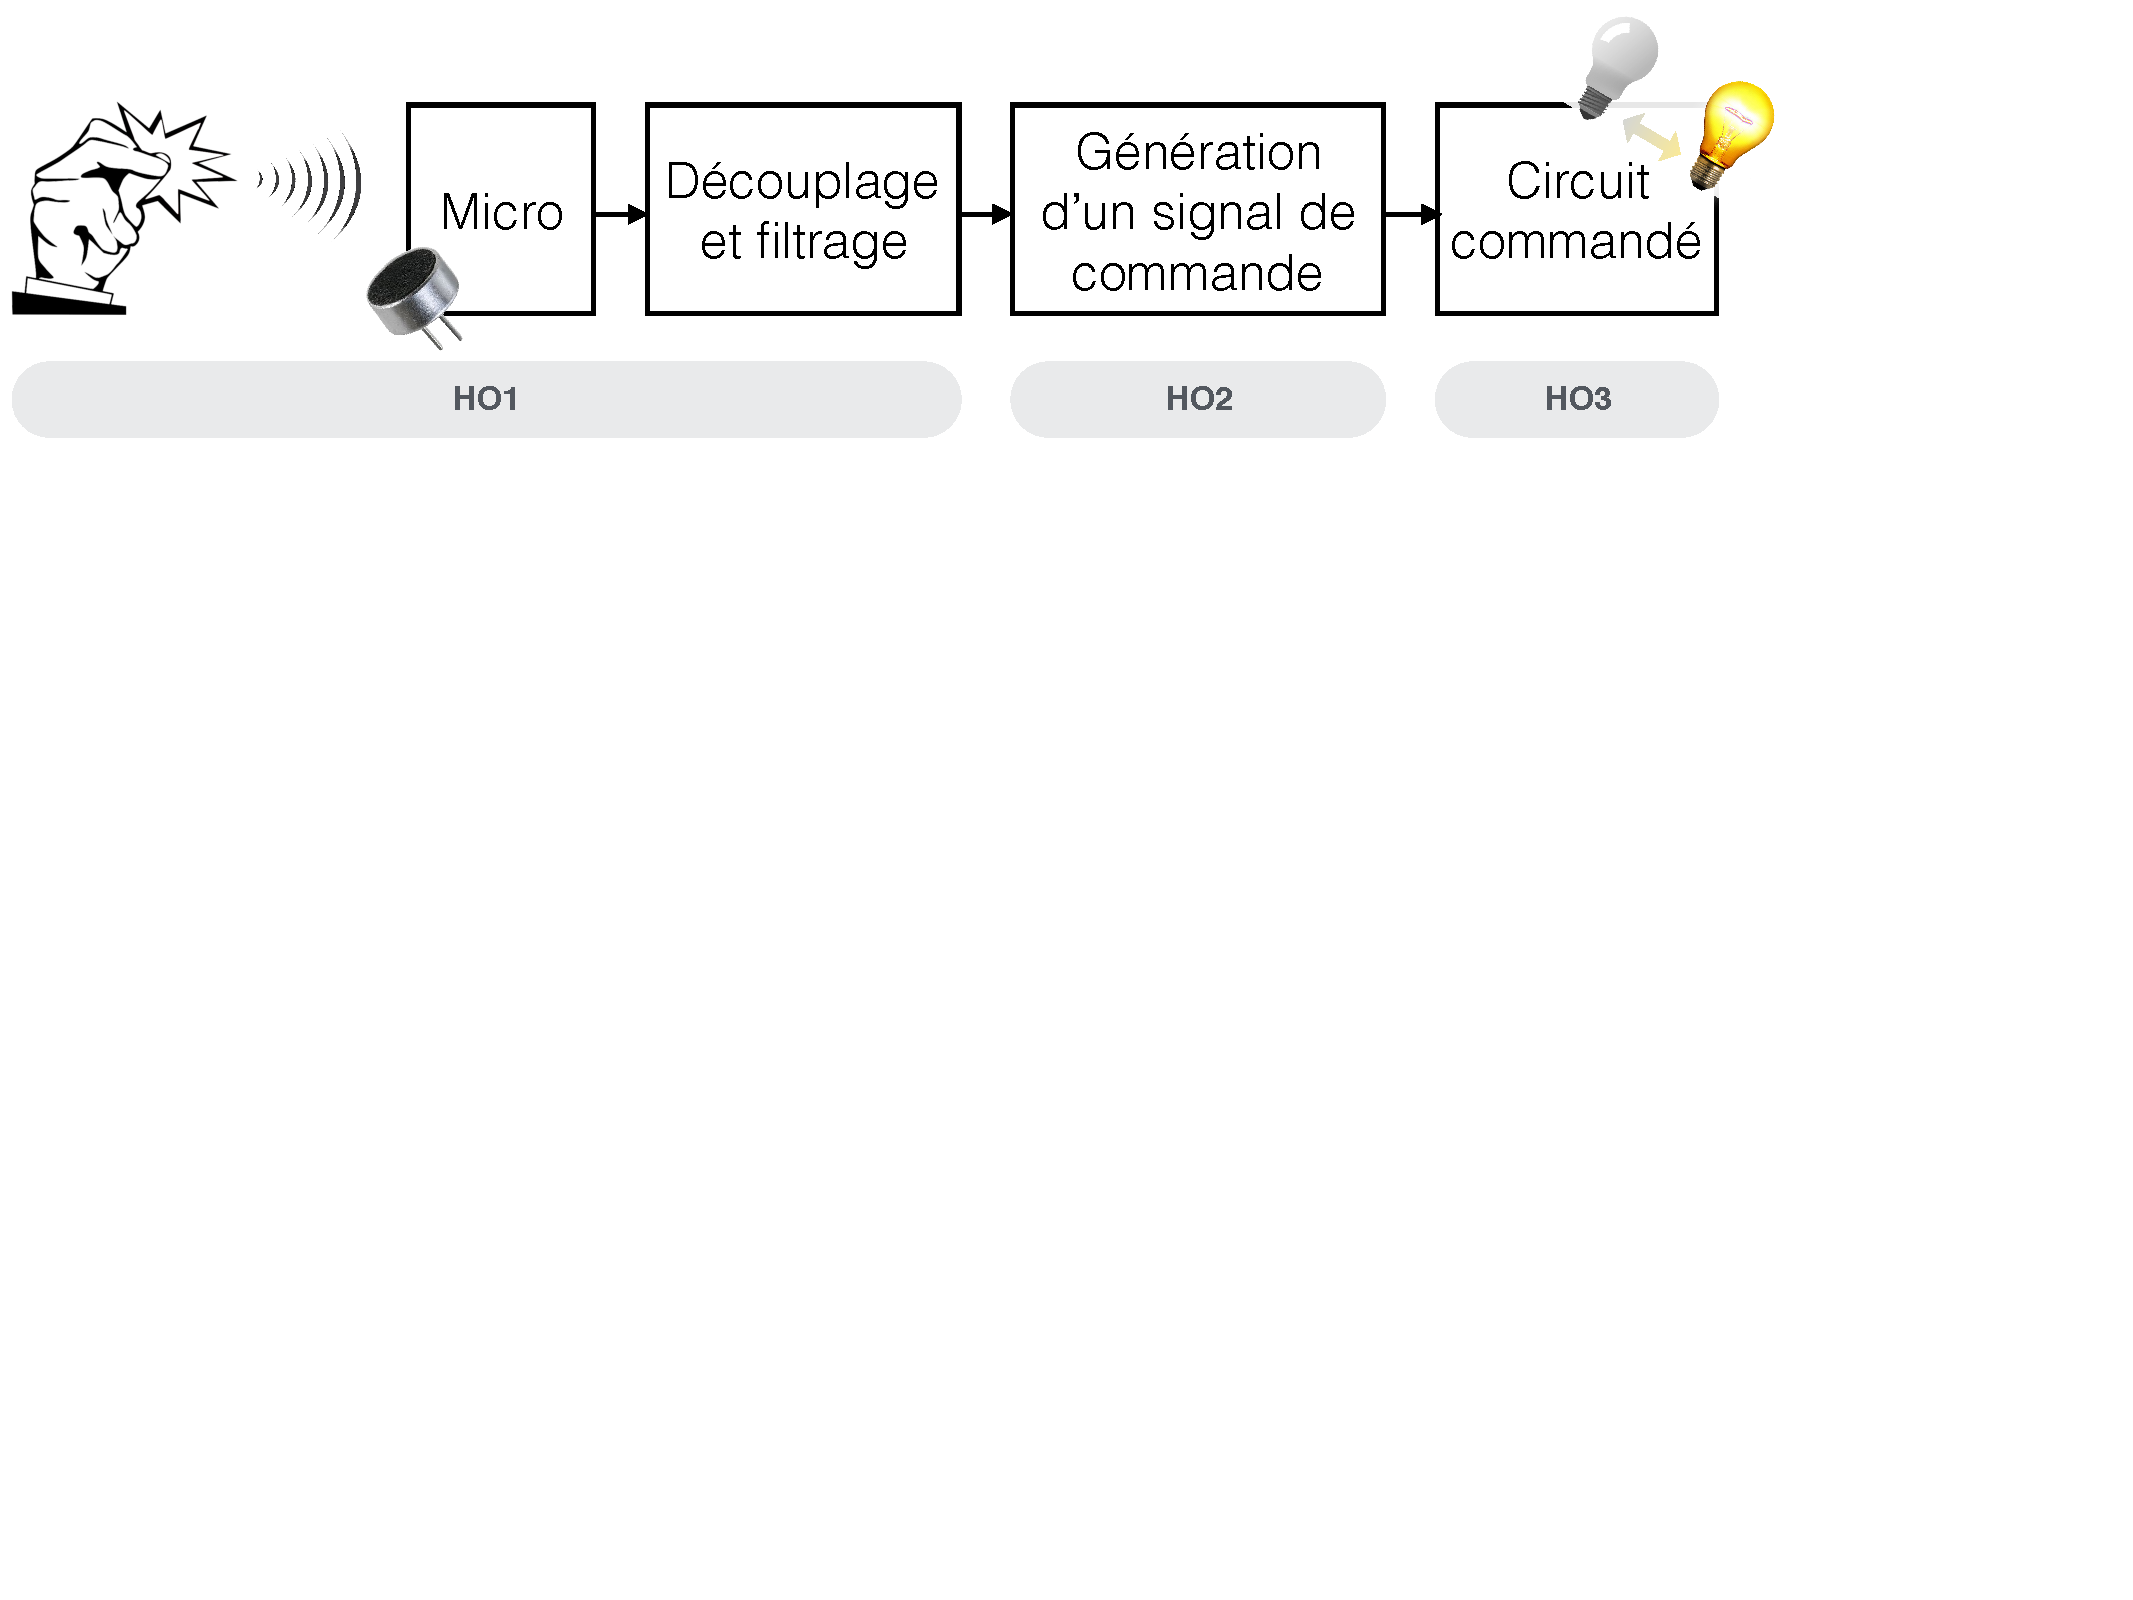
\includegraphics[width=0.8\textwidth]{figures/SchemaBloc.pdf}
	\caption{Schéma-bloc du circuit.}
	\label{fig:block-diagram}
\end{figure}

\vspace{1cm}

Les objectifs de ce troisième hands-on (HO3) sont:

\begin{itemize}
    \item[-] D'utiliser le matériel mis à disposition (i.g. oscilloscope, multimètre, etc ...) afin de vérifier les composants et les signaux d'intérêt
	\item[-] De comprendre l'utilité d'un registre pour créer une mémoire
	\item[-] De savoir le connecter pour créer une bascule
    \item[-] D'utiliser un transistor pour contrôler un circuit.
\end{itemize}

Durant cet HO3, vous allez commencer avec la compréhension des registres pour pouvoir reproduire les signaux de la Figure~\ref{fig:signal-all_HO3}. Ensuite, vous allez placer un transistor pour allumer ou éteindre la LED. A la fin de cette séance, le circuit complet ressemblera à la Figure~\ref{fig:all}. Vous serez arrivés au bout de ce projet-éclair. 
\vspace{1.5cm}

\begin{figure}[h!]
    \centering
    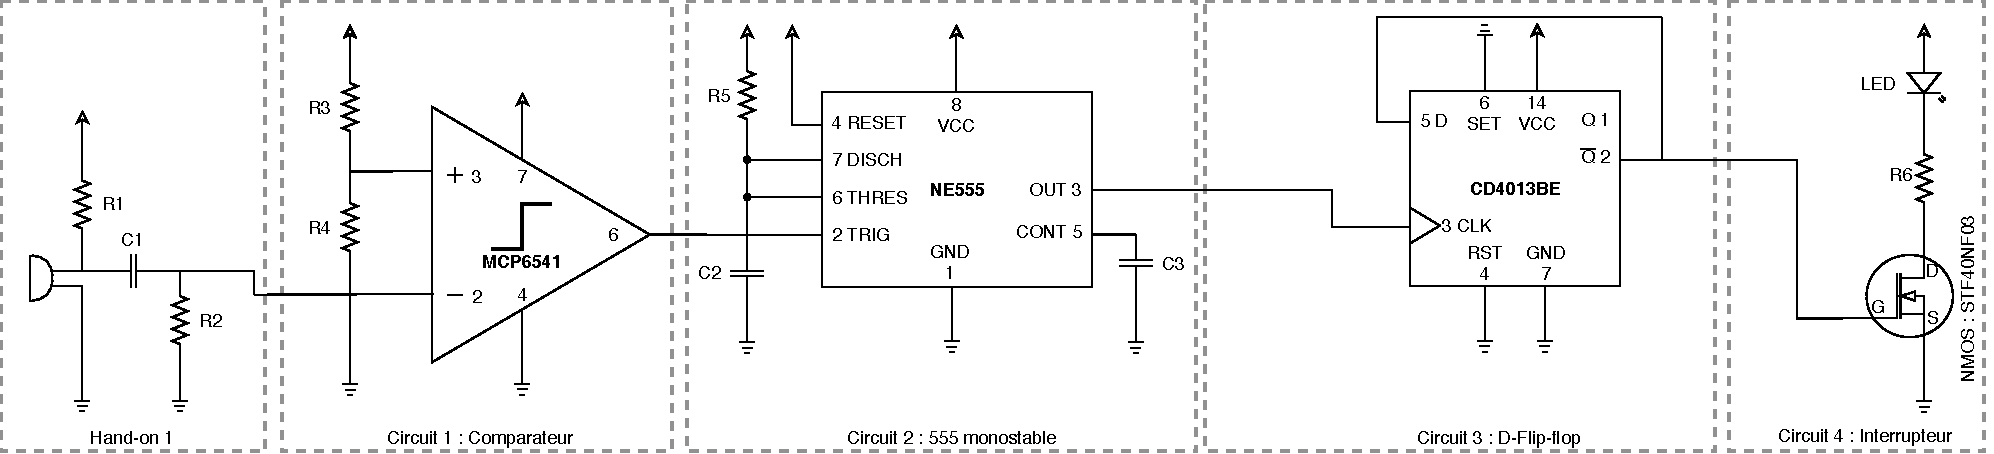
\includegraphics[width=1\textwidth]{HO3_complete.pdf}
    \caption{Circuit complet du Clap Hand Sensor}
    \label{fig:all}
\end{figure}